\documentclass{article}
\usepackage[utf8]{inputenc}
\usepackage{geometry}
\usepackage{graphicx}
\usepackage{hyperref}

\geometry{ left=25mm, right=25mm, top=20mm, bottom=25mm }

\title{\textbf{Report N°3 MSc Thesis: Active Constraints}}
\author{\textbf{Alberto Rota} - \textit{Supervisor: Prof. Elena De Momi}}
\date{}


\begin{document}
\maketitle
\paragraph{Title:} \textit{To Be Defined}
\section*{General guidelines}
    Development of surgical training tasks implementing Active Constraints of
    different nature and with different levels of intervention, in order to
    evaluate their efficacy and role in Robot-Assisted Minimally Invasive
    Surgery.
    \begin{itemize}
        \item \textit{Phase 1: }Software Development in a virtual environment
        (Unity)
        \item \textit{Phase 2: }Implementing on the dVRK, followed by experimental tests with data gathering, analysis and validation
    \end{itemize}
\section*{Work Planned from the previous report}
    \begin{itemize}
        \item Implementing the last few remaining virtual fixtures described in
        "Active Constraints/Virtual Fixtures: A survey" and in the related
        literature
        \item Creating at least one functional surgical task in the virtual
        environment in Unity
    \end{itemize}
\section*{Progress}
    \begin{itemize}
        \item Learned the Unity Physics Engine with the rigid body physics,
        collisions and dynamics
        \item The Unity scene now saves all the relevant data about each task
        and about the virtual fixtures employed: end-effector position,
        orientation, velocity, force feedback, distance from
        trajectory/obstacles, \textit{etc.}
        \item Built a rudimentary surgical task between Blender (for 3D
        modelling) and Unity, in order to test the rigid body behavior. The task
        is complemented with one of the virtual fixtures implemented before, the
        \textit{Trajectory Guidance Active Constraint}. A screenshot of the task
        is reported in the following page.
        
        For this very rudimentary task, the user controls only the orange
        "scoop" and he has to pick up and carry the blue sphere from the green
        block to the yellow one. The 4 red points define the reference 
        trajectory (in green)
        that the user has to follow. The virtual fixture calculates the force
        that will be provided as haptic feedback (not visible in the picture, the "scoop" stands still while taking the screenshot).
        
        The simulation is completely functional and data for each "trial" of the
        task is saved for analysis, plotting and evaluation
        
    \end{itemize}
    
    \section*{Next Steps}
    \begin{itemize}
        \item Literature research on surgical tasks: what to aim at and what to
        focus on when building one
        \item From the rudimentary task alredy implemented, create more complex
        ones that will allow to employ the different types of virtual fixtures.
        \newline NOTE: Anywhere possible, the virtual objects employed will be 3D models
        of organs, and the end-effector will be replaced by the PSM tooltip
    \end{itemize}
    
    \newpage
    \section*{Screenshots}
    \begin{figure}[h!]
            \begin{center}
                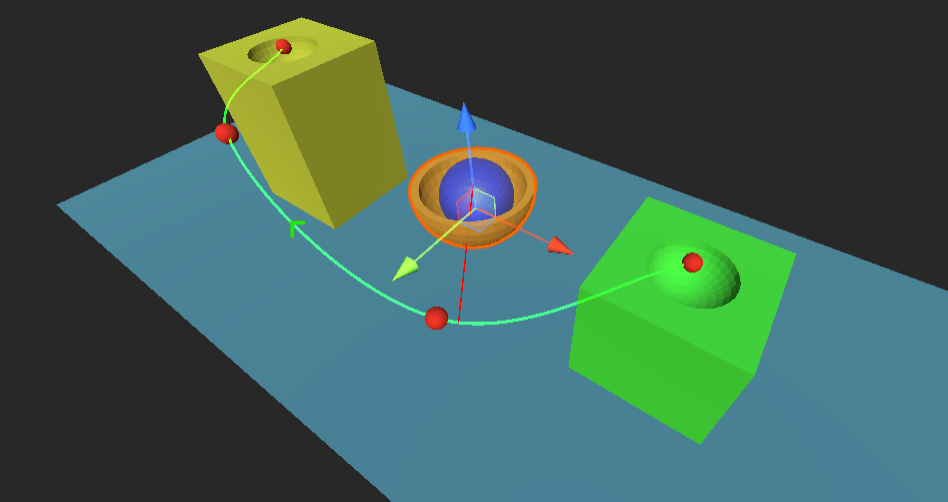
\includegraphics[width=\textwidth]{scene.png}
            \end{center}
    \end{figure}
    % \begin{figure}[h!] \begin{small} \begin{center}
        %     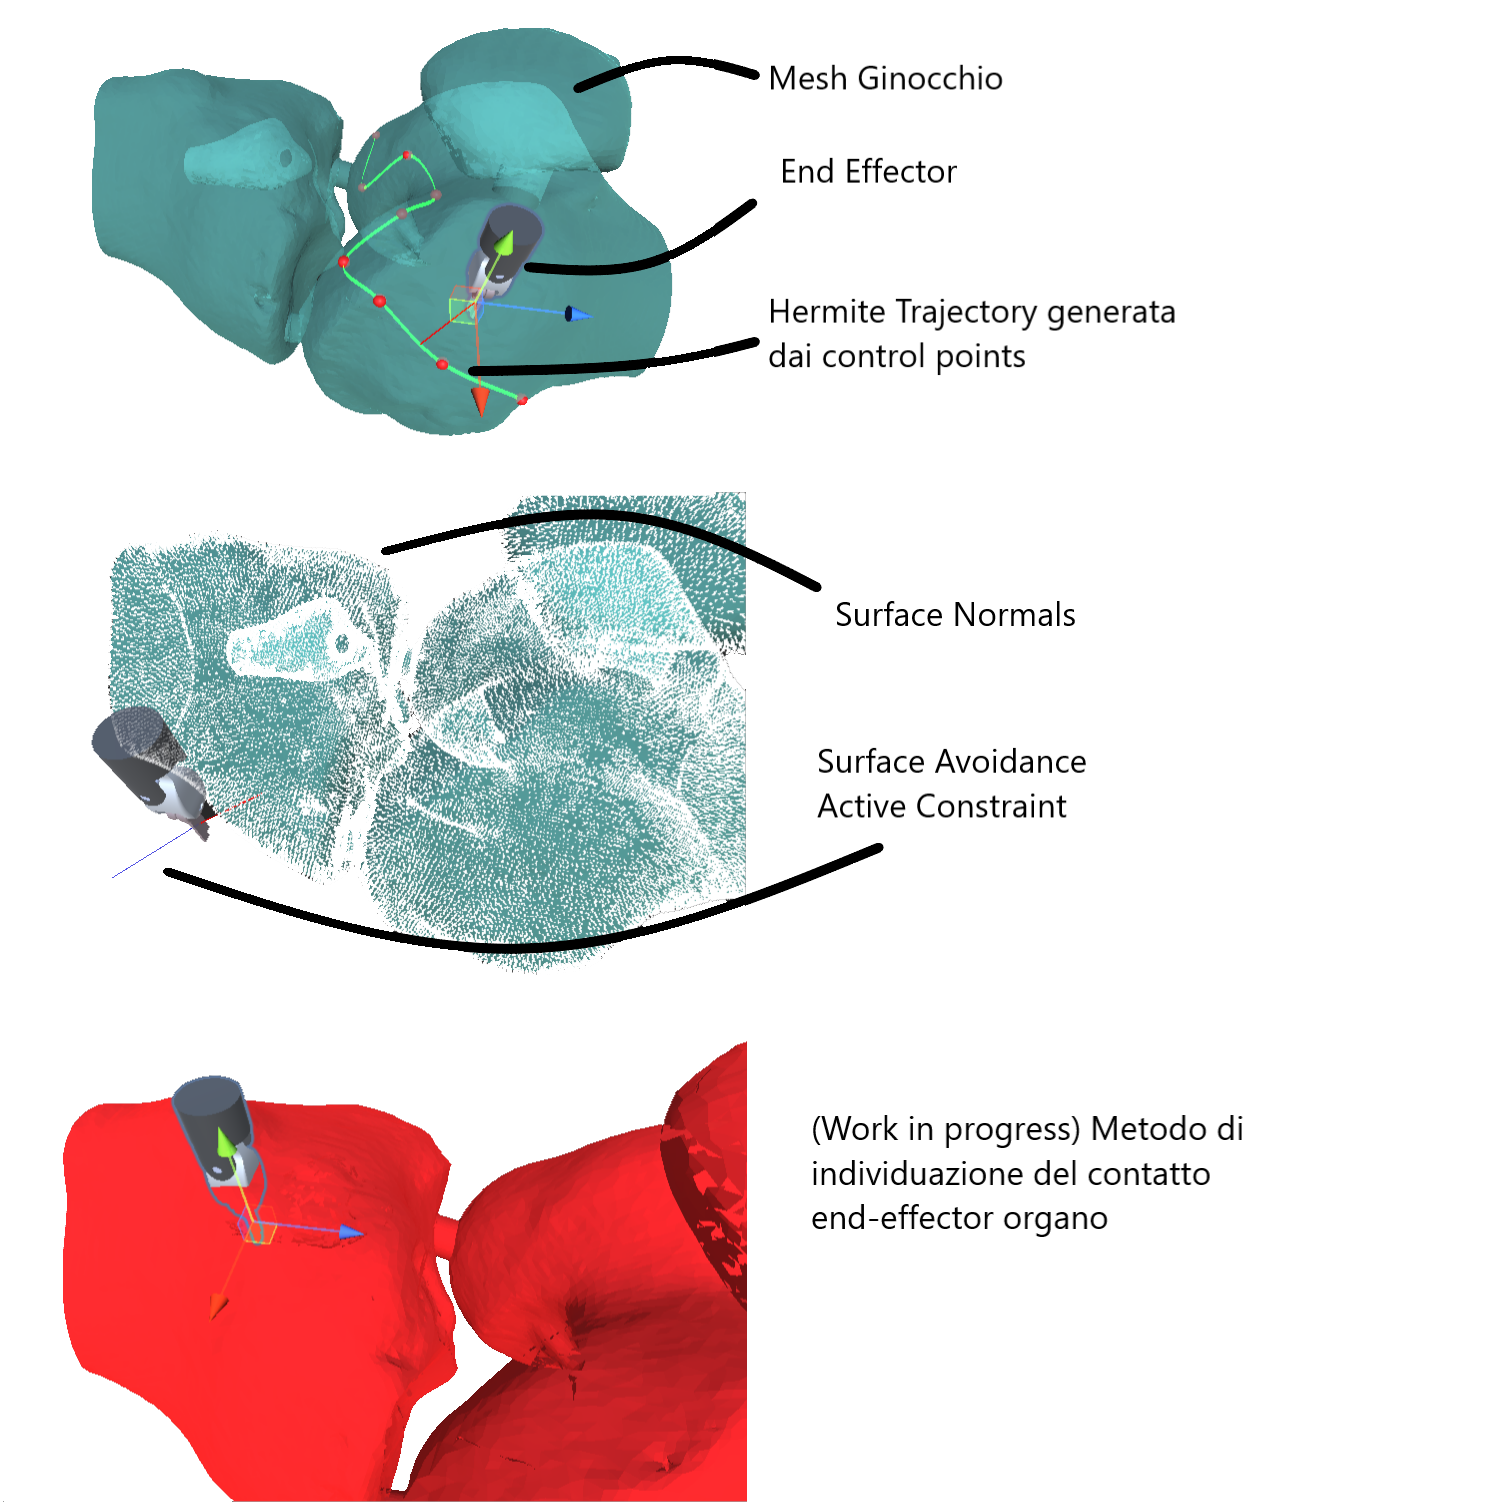
\includegraphics[width=0.95\textwidth]{Scene.png} \end{center}
%     \label{fig:} \end{small} \end{figure}

    
\end{document}